\documentclass{beamer}

\usepackage[utf8]{inputenc}
\usepackage{minted}
\usepackage{listings}
\usepackage{graphicx}
\usepackage{xcolor}
\usepackage{adjustbox}


\usetheme{Madrid}
\useinnertheme{circles}
\definecolor{ssgreen}{HTML}{669B41}
\usecolortheme[named=ssgreen]{structure}
\setbeamertemplate{navigation symbols}{}

\AtBeginEnvironment{frame}{\setcounter{footnote}{0}}

\title[Kubernetes]{Introduction to Kubernetes}
\author[Ed MacDonald]{Ed MacDonald\\emacdonald@solutionstreet.com}
\institute[\href{https://solutionstreet.com}{SolutionStreet}]{SolutionStreet\\\href{https://solutionstreet.com}{(solutionstreet.com)}}
\date{July 2020}

\titlegraphic{ \includegraphics[width=2cm]{logo} }

\begin{document}
\frame{\titlepage}

\begin{frame}
\frametitle{A Note on Capitalization}

I agonized over which words to capitalize.

\begin{itemize}
   \item{I wanted to capitalize ``things" that were important concepts in the Kubernetes domain:}
   \begin{itemize}
      \item{Any Kubernetes component: Deployment, Pod, ReplicaSet, StatefulSet, ...}
      \item{Application, Container, Kubernetes, Node, Volume}
   \end{itemize}

   \item{But some didn't quite make the cut:}
   \begin{itemize}
      \item{cluster, component}
   \end{itemize}

   \item{And I couldn't bring myself to capitalize things I type at the Unix command line:}
   \begin{itemize}
      \item{docker, helm, kubectl, minikube}
   \end{itemize}
\end{itemize}

If you disagree, let's agree to disagree and move on.

\end{frame}

\begin{frame}
\frametitle{What is Kubernetes?}
\begin{itemize}
    \item{A Container Orchestration Framework.}
    \item{Very well suited for Applications that scale horizontally (stateless).}
    \item{But can also accommodate portions of your infrastructure that do not scale horizontally (stateful). Don't let people tell you otherwise.}
\end{itemize}
\end{frame}

\begin{frame}
    \frametitle{How do you use it?}
    \begin{itemize}
        \item{Package your Application components as Containers.}
        \item{Run the Containers on Kubernetes Pods.}
        \item{Let Kubernetes manage the Pods for you!}
    \end{itemize}
\end{frame}

\begin{frame}
    \frametitle{Why go through the hassle? (It can be a hassle)}
    Kubernetes can manage resources for you by:
    \begin{itemize}
        \item{Changing the number of running Pods to meet traffic demands.}
        \item{Adjusting compute resources to meet compute demands.}
        \item{Replacing unresponsive Pods with new ones.}
    \end{itemize}
\end{frame}

\begin{frame}
    \begin{center}
        \Huge High Level Deployment Walkthrough
    \end{center}
\end{frame}

\begin{frame}
    \frametitle{Deploying An App: Build Your App}
    \includegraphics[width=\textwidth,height=0.85\textheight,keepaspectratio]{graphics/deploy-00-app.eps}
\end{frame}

\begin{frame}
    \frametitle{Deploying An App: Package Your App as a Container}
    \includegraphics[width=\textwidth,height=0.85\textheight,keepaspectratio]{graphics/deploy-01-appContainerized.eps}
\end{frame}

\begin{frame}
    \frametitle{Deploying An App: Push The Container to a Repository}
    \includegraphics[width=\textwidth,height=0.85\textheight,keepaspectratio]{graphics/deploy-02-containerToRepo.eps}
\end{frame}

\begin{frame}
    \frametitle{Deploying An App: Deploy Pods to a Kubernetes Cluster}
    \includegraphics[width=\textwidth,height=0.85\textheight,keepaspectratio]{graphics/deploy-03-emptyPods.eps}
\end{frame}

\begin{frame}
    \frametitle{Deploying An App: Pods Pull Your Container}
    \includegraphics[width=\textwidth,height=0.85\textheight,keepaspectratio]{graphics/deploy-04-podsWithContainers.eps}
\end{frame}

\begin{frame}
    \begin{center}
        \Huge Simple, right? Now let's get into the weeds.
    \end{center}
\end{frame}

\begin{frame}
    \frametitle{Kubernetes Nodes}
    \begin{itemize}
        \item The (virtual) machines that make up the Kubernetes cluster.
        \item Kubernetes schedules Pods to run on these Nodes.
        \item Kubernetes can change the number of Nodes to increase/decrease compute resources.
    \end{itemize}
\end{frame}

\begin{frame}
    \frametitle{Tool: minikube\footnotemark}
    \begin{itemize}
        \item Easiest way to install a (single Node) Kubernetes cluster on your machine.
        \item For development purposes only!
    \end{itemize}
    \footnotetext[1]{https://kubernetes.io/docs/tasks/tools/install-minikube}
\end{frame}

% https://www.patrickbaylis.com/posts/2018-10-11-beamer-resizing/
\begin{frame}
    \frametitle{Kubernetes Nodes}
    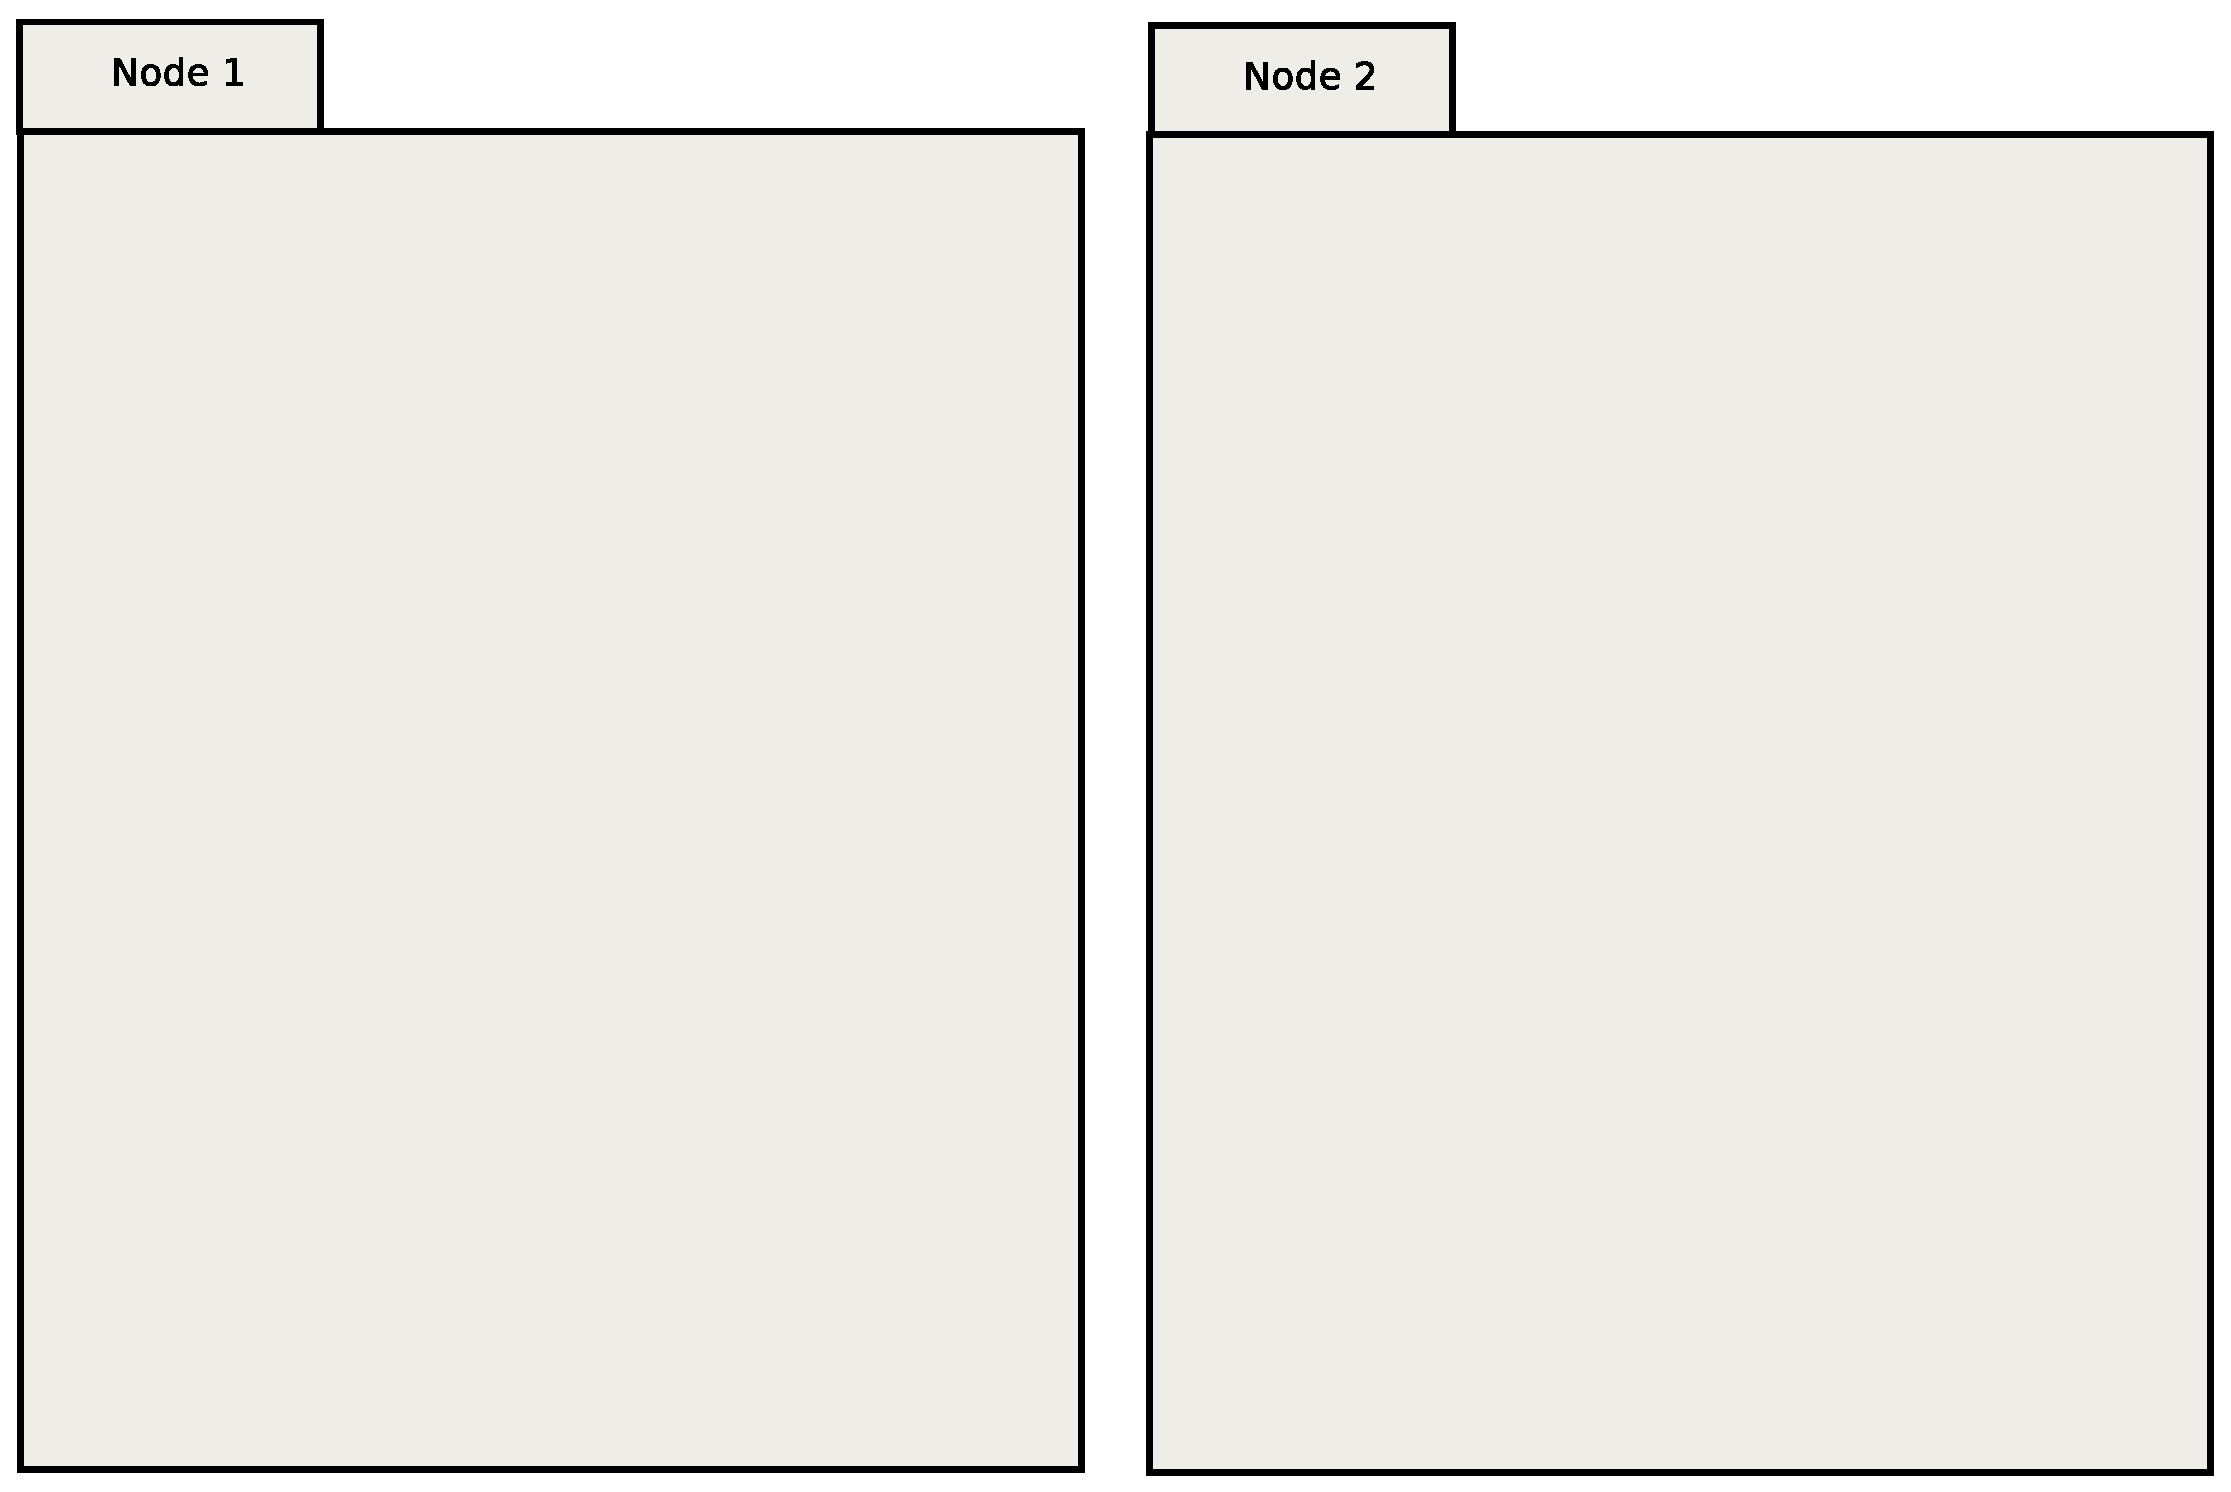
\includegraphics[width=\textwidth,height=0.85\textheight,keepaspectratio]{graphics/00-nodes.eps}
\end{frame}

\begin{frame}
    \frametitle{Pods}
    Pods (not Containers!) are the fundamental building blocks of a Kubernetes Application
    \begin{itemize}
        \item A Pod is a group of one or more Containers that work closely together on a specific task.
        \item Pods manage Volumes for their Containers.
        \item Pods specify health check endpoints for their Containers.
        \item Kubernetes software is deployed as Pods on the cluster!
    \end{itemize}
\end{frame}

\begin{frame}
    \frametitle{System Pods}
    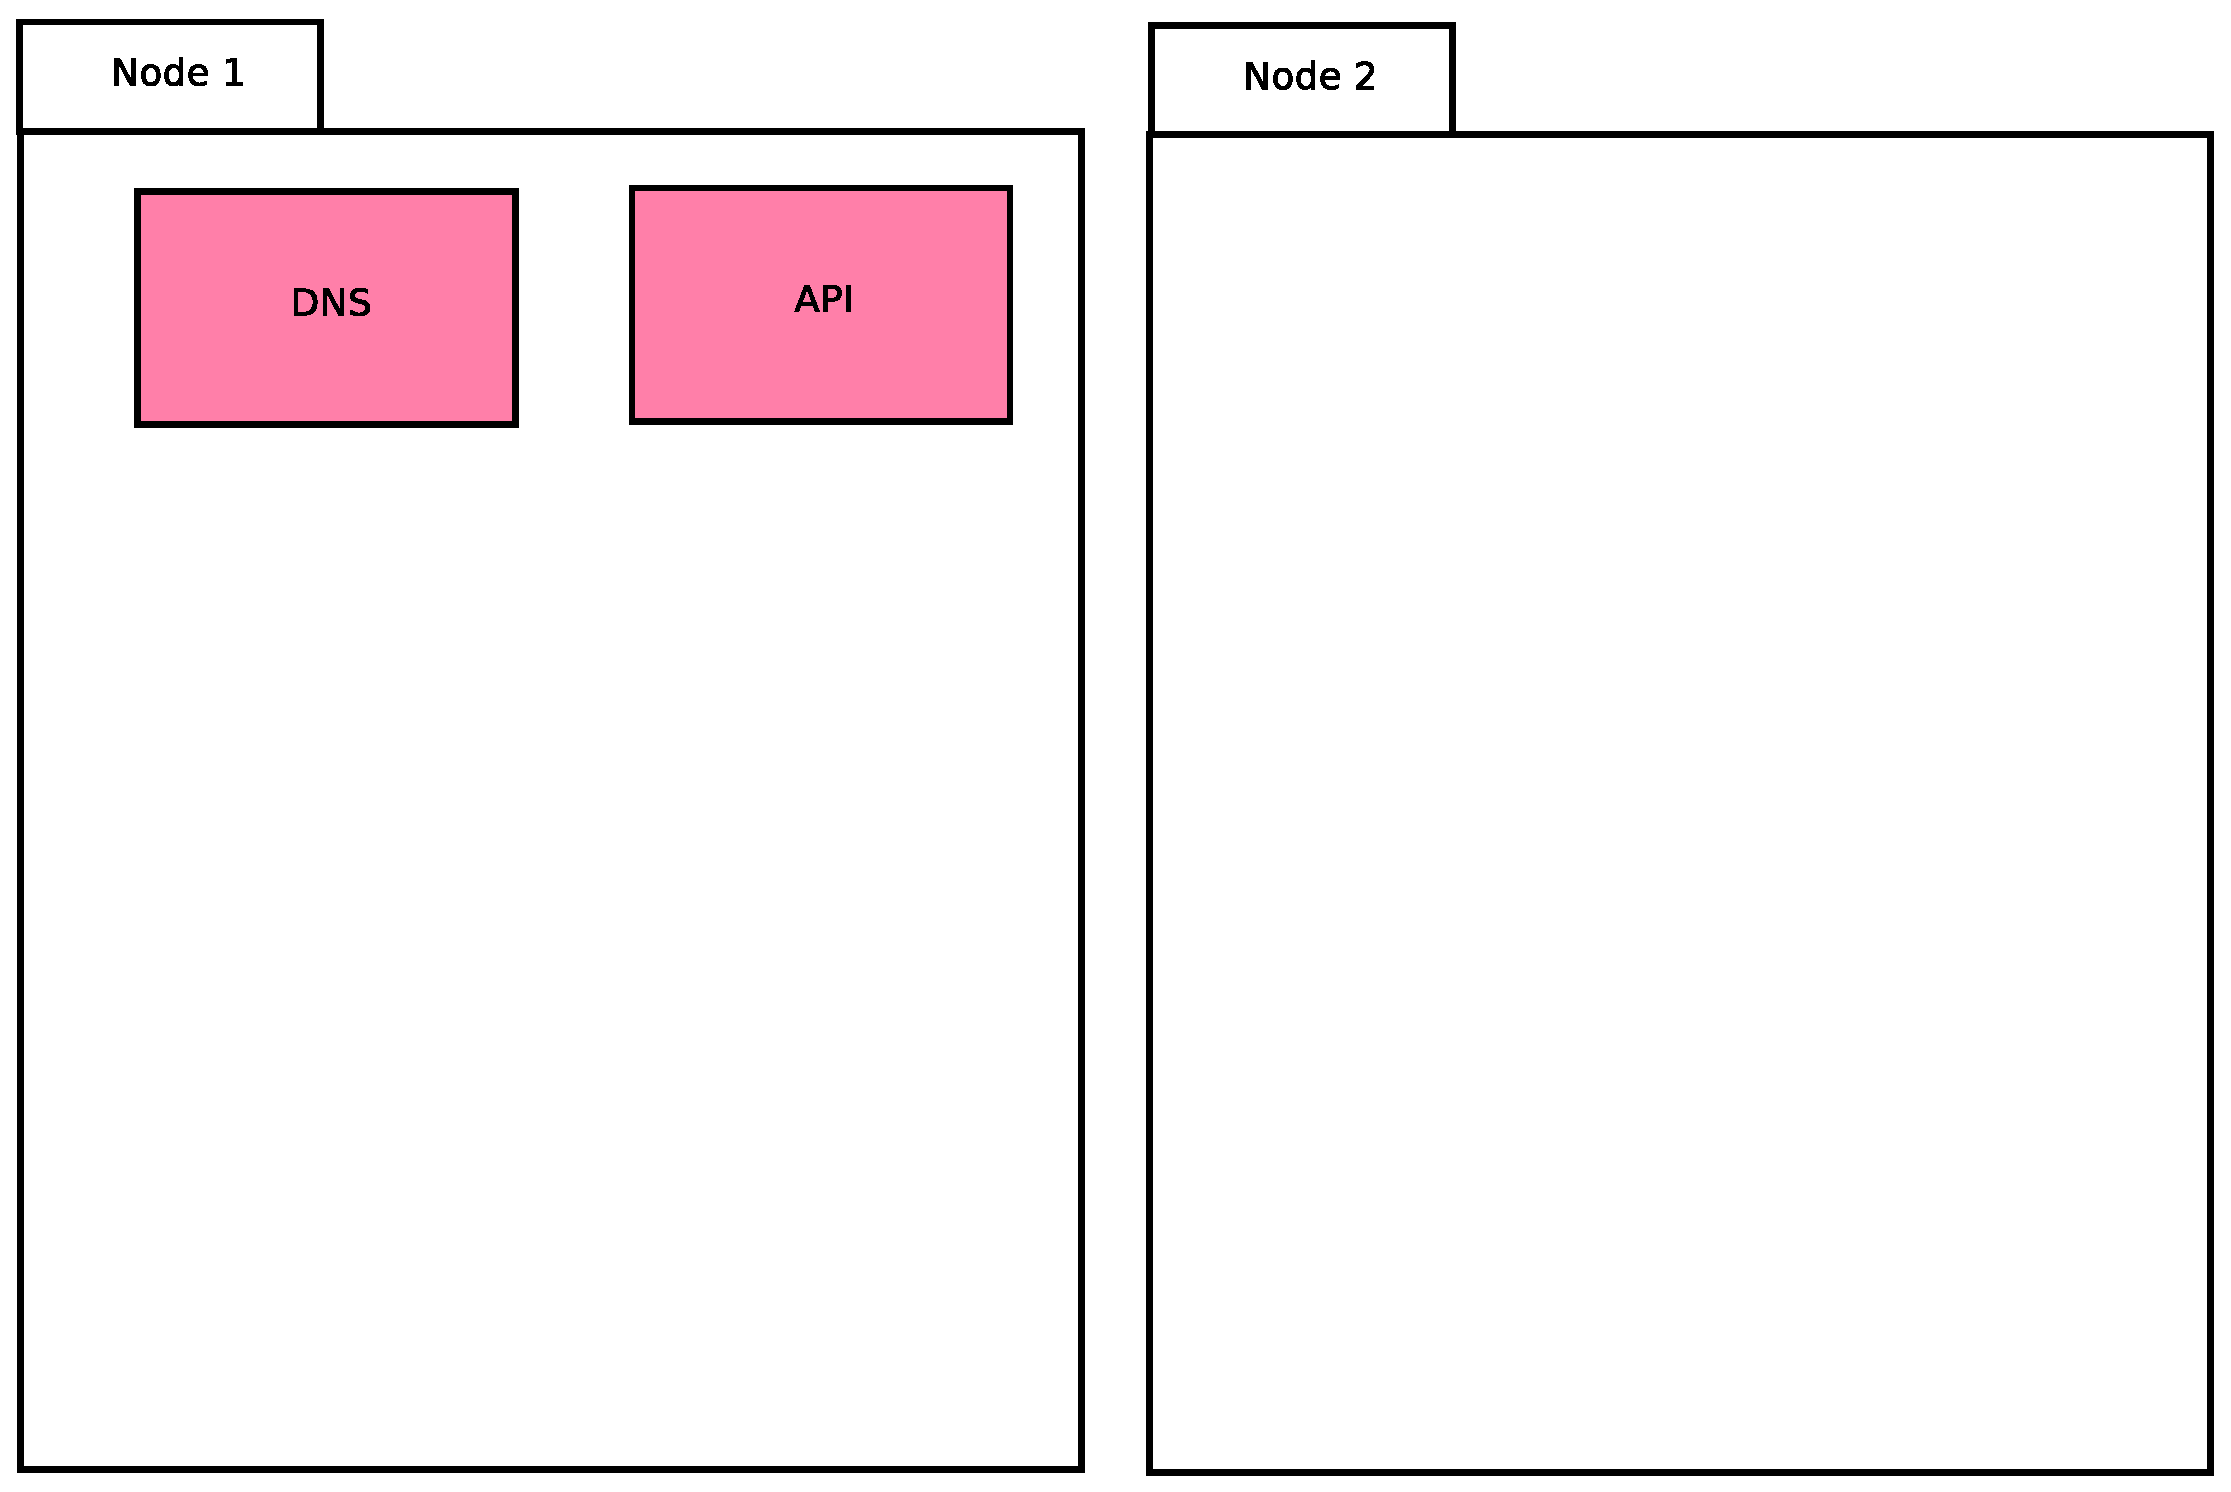
\includegraphics[width=\textwidth,height=0.85\textheight,keepaspectratio]{graphics/01-systemPods.eps}
\end{frame}

\begin{frame}
    \frametitle{The Sample Apps}
    I wrote two Applications that do nothing other than suggest a random Subreddit.
    \begin{itemize}
        \item One is stateless and selects at random from a list of 280 Subreddits.
        \begin{itemize}
            \item The list never changes.
            \item It doesn't need to store anything anywhere.
        \end{itemize}
        \item One is stateful and removes each Subreddit from the list upon suggesting it.
        \begin{itemize}
            \item It removes the selected Subreddit from the list.
            \item Persists the list.
            \item Uses the updated list to service the next request.
        \end{itemize}
    \end{itemize}
\end{frame}

\begin{frame}
    \frametitle{An Aside on Pods}
    \begin{itemize}
        \item Pods come and go.
        \begin{itemize}
            \item They can be replaced if unresponsive.
            \item They can be deleted on one Node and added on another (moved).
            \item \textbf{You cannot prevent either of these things from happening.}
        \end{itemize}
        \item By default, when Pods are replaced or moved, the Volumes they get won't be the ones they had before.
        \item By default, they'll also have new hostnames.
        \item Not a big deal for stateless Applications.
        \item Definitely something that needs to be addressed for our stateful Application, though.
    \end{itemize}
\end{frame}

\begin{frame}
    \frametitle{Tool: docker\footnotemark}
    \begin{itemize}
        \item Our Applications need to be packaged as docker Containers.
        \item We need to be able to build our Containers and publish them to minikube's docker server.
    \end{itemize}
    \footnotetext[1]{https://www.docker.com/get-started}
\end{frame}

\begin{frame}
    \frametitle{Stateless Application Pods}
    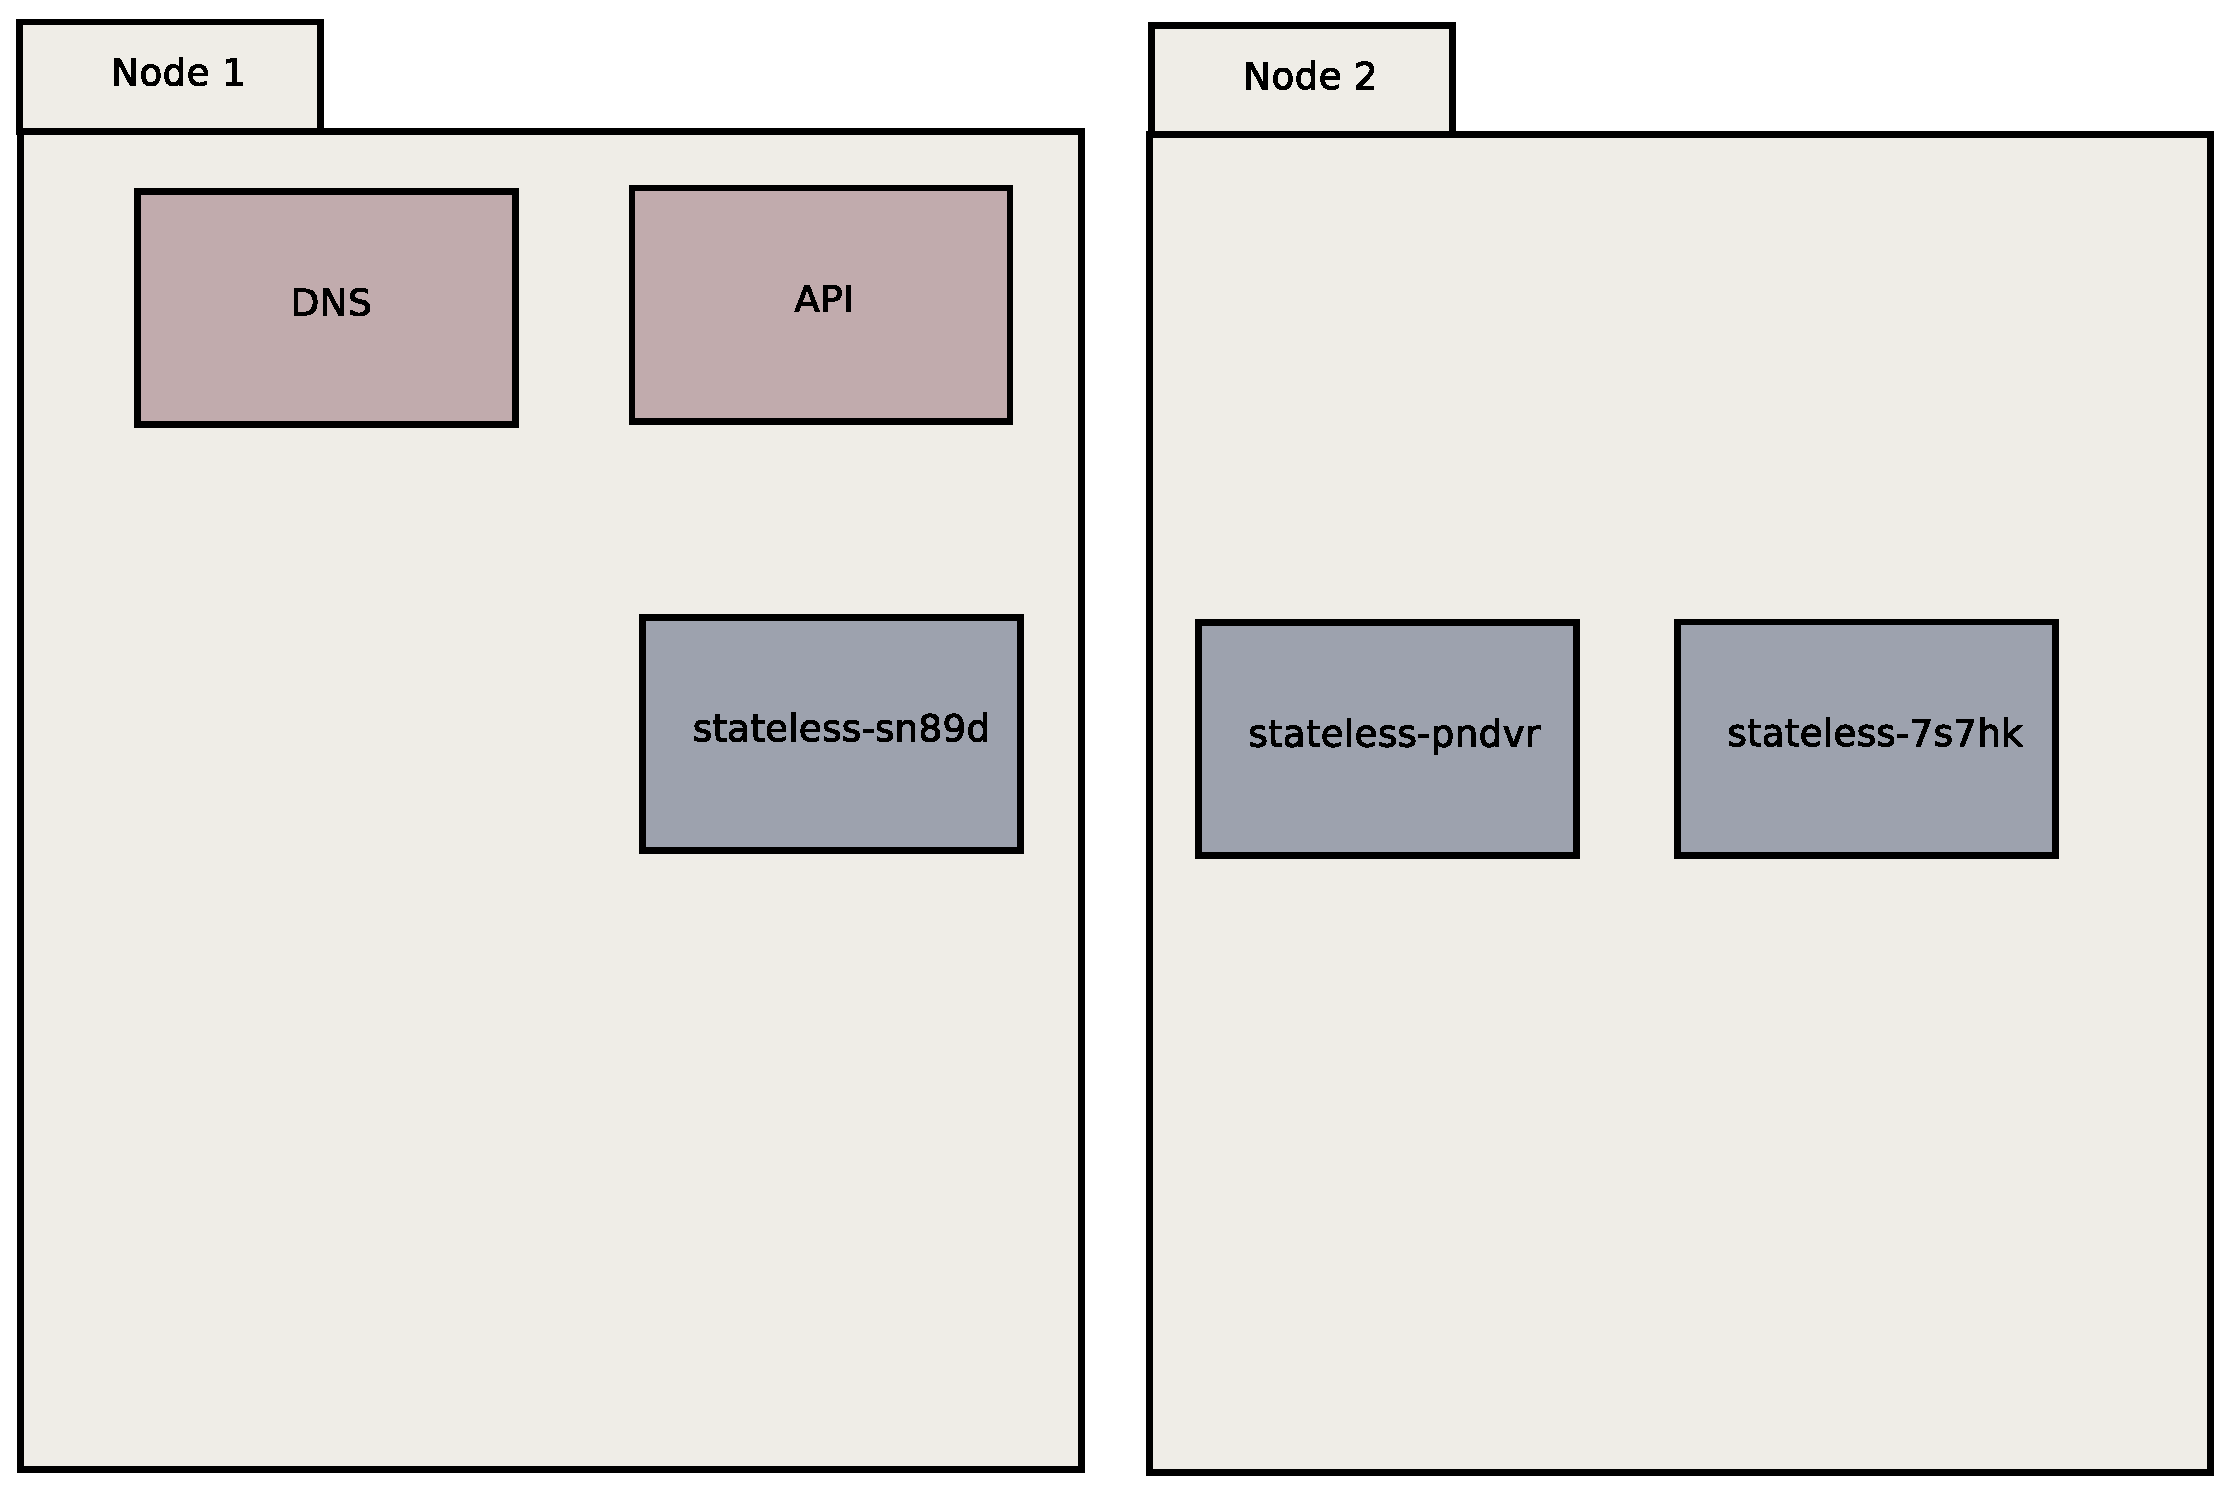
\includegraphics[width=\textwidth,height=0.85\textheight,keepaspectratio]{graphics/02-statelessAppPods.eps}
\end{frame}

\begin{frame}
    \frametitle{Stateful Application Pods}
    \includegraphics[width=\textwidth,height=0.85\textheight,keepaspectratio]{graphics/03-statefulAppPods.eps}
\end{frame}

\begin{frame}
    \frametitle{Controllers}
    \begin{itemize}
        \item Don't create Pods directly.
        \item Instead, create a Controller that manages the Pods for you.
    \end{itemize}
\end{frame}

\begin{frame}
    \frametitle{Controllers: ReplicaSets}
    \begin{itemize}
        \item State how many Pods you want.
        \item Pods are treated as if they were stateless.
        \item From Application's point of view, Pods in a ReplicaSet are indistinguishable.
    \end{itemize}
\end{frame}

\begin{frame}
    \frametitle{Controllers: Deployments}
    \begin{itemize}
        \item ReplicaSets with more features.
        \item I'm not going to use those features (I'm honestly not sure what they are).
        \item But I use Deployments because helm produces them for skeleton helm projects.
    \end{itemize}
\end{frame}

\begin{frame}
    \frametitle{Controllers: StatefulSets}
    StatefulSets manage Pods that are required to have state, namely:
    \begin{itemize}
        \item Pods in a StatefulSet each have a persistent network identity.
        \item Pods in a StatefulSet each have persistent storage.
        \item Persistent here means they stay the same when Pods are replaced or moved. You can stop worrying about our stateful Application now.
    \end{itemize}
\end{frame}

\begin{frame}
\frametitle{Tool: kubectl\footnotemark}
\begin{itemize}
\item We need to be able to communicate with our cluster.
\item kbuectl can update components in our cluster.
\item kbuectl can inspect components in our cluster.
\item kbuectl can create components in our cluster, but we'll use another tool for that...
\end{itemize}
\footnotetext[1]{https://kubernetes.io/docs/tasks/tools/install-kubectl}
\end{frame}

\begin{frame}
\frametitle{Tool: helm\footnotemark}
\begin{itemize}
    \item Tool for packaging and deploying Kubernetes Applications.
    \item We'll use helm (instead of kubectl) to create our Kubernetes components.
\end{itemize}
\footnotetext[1]{\href{https://helm.sh}{https://helm.sh}}
\end{frame}

\begin{frame}
    \frametitle{Deployment}
    \includegraphics[width=\textwidth,height=0.85\textheight,keepaspectratio]{graphics/04-deployment.eps}
\end{frame}

\begin{frame}
    \frametitle{StatefulSet}
    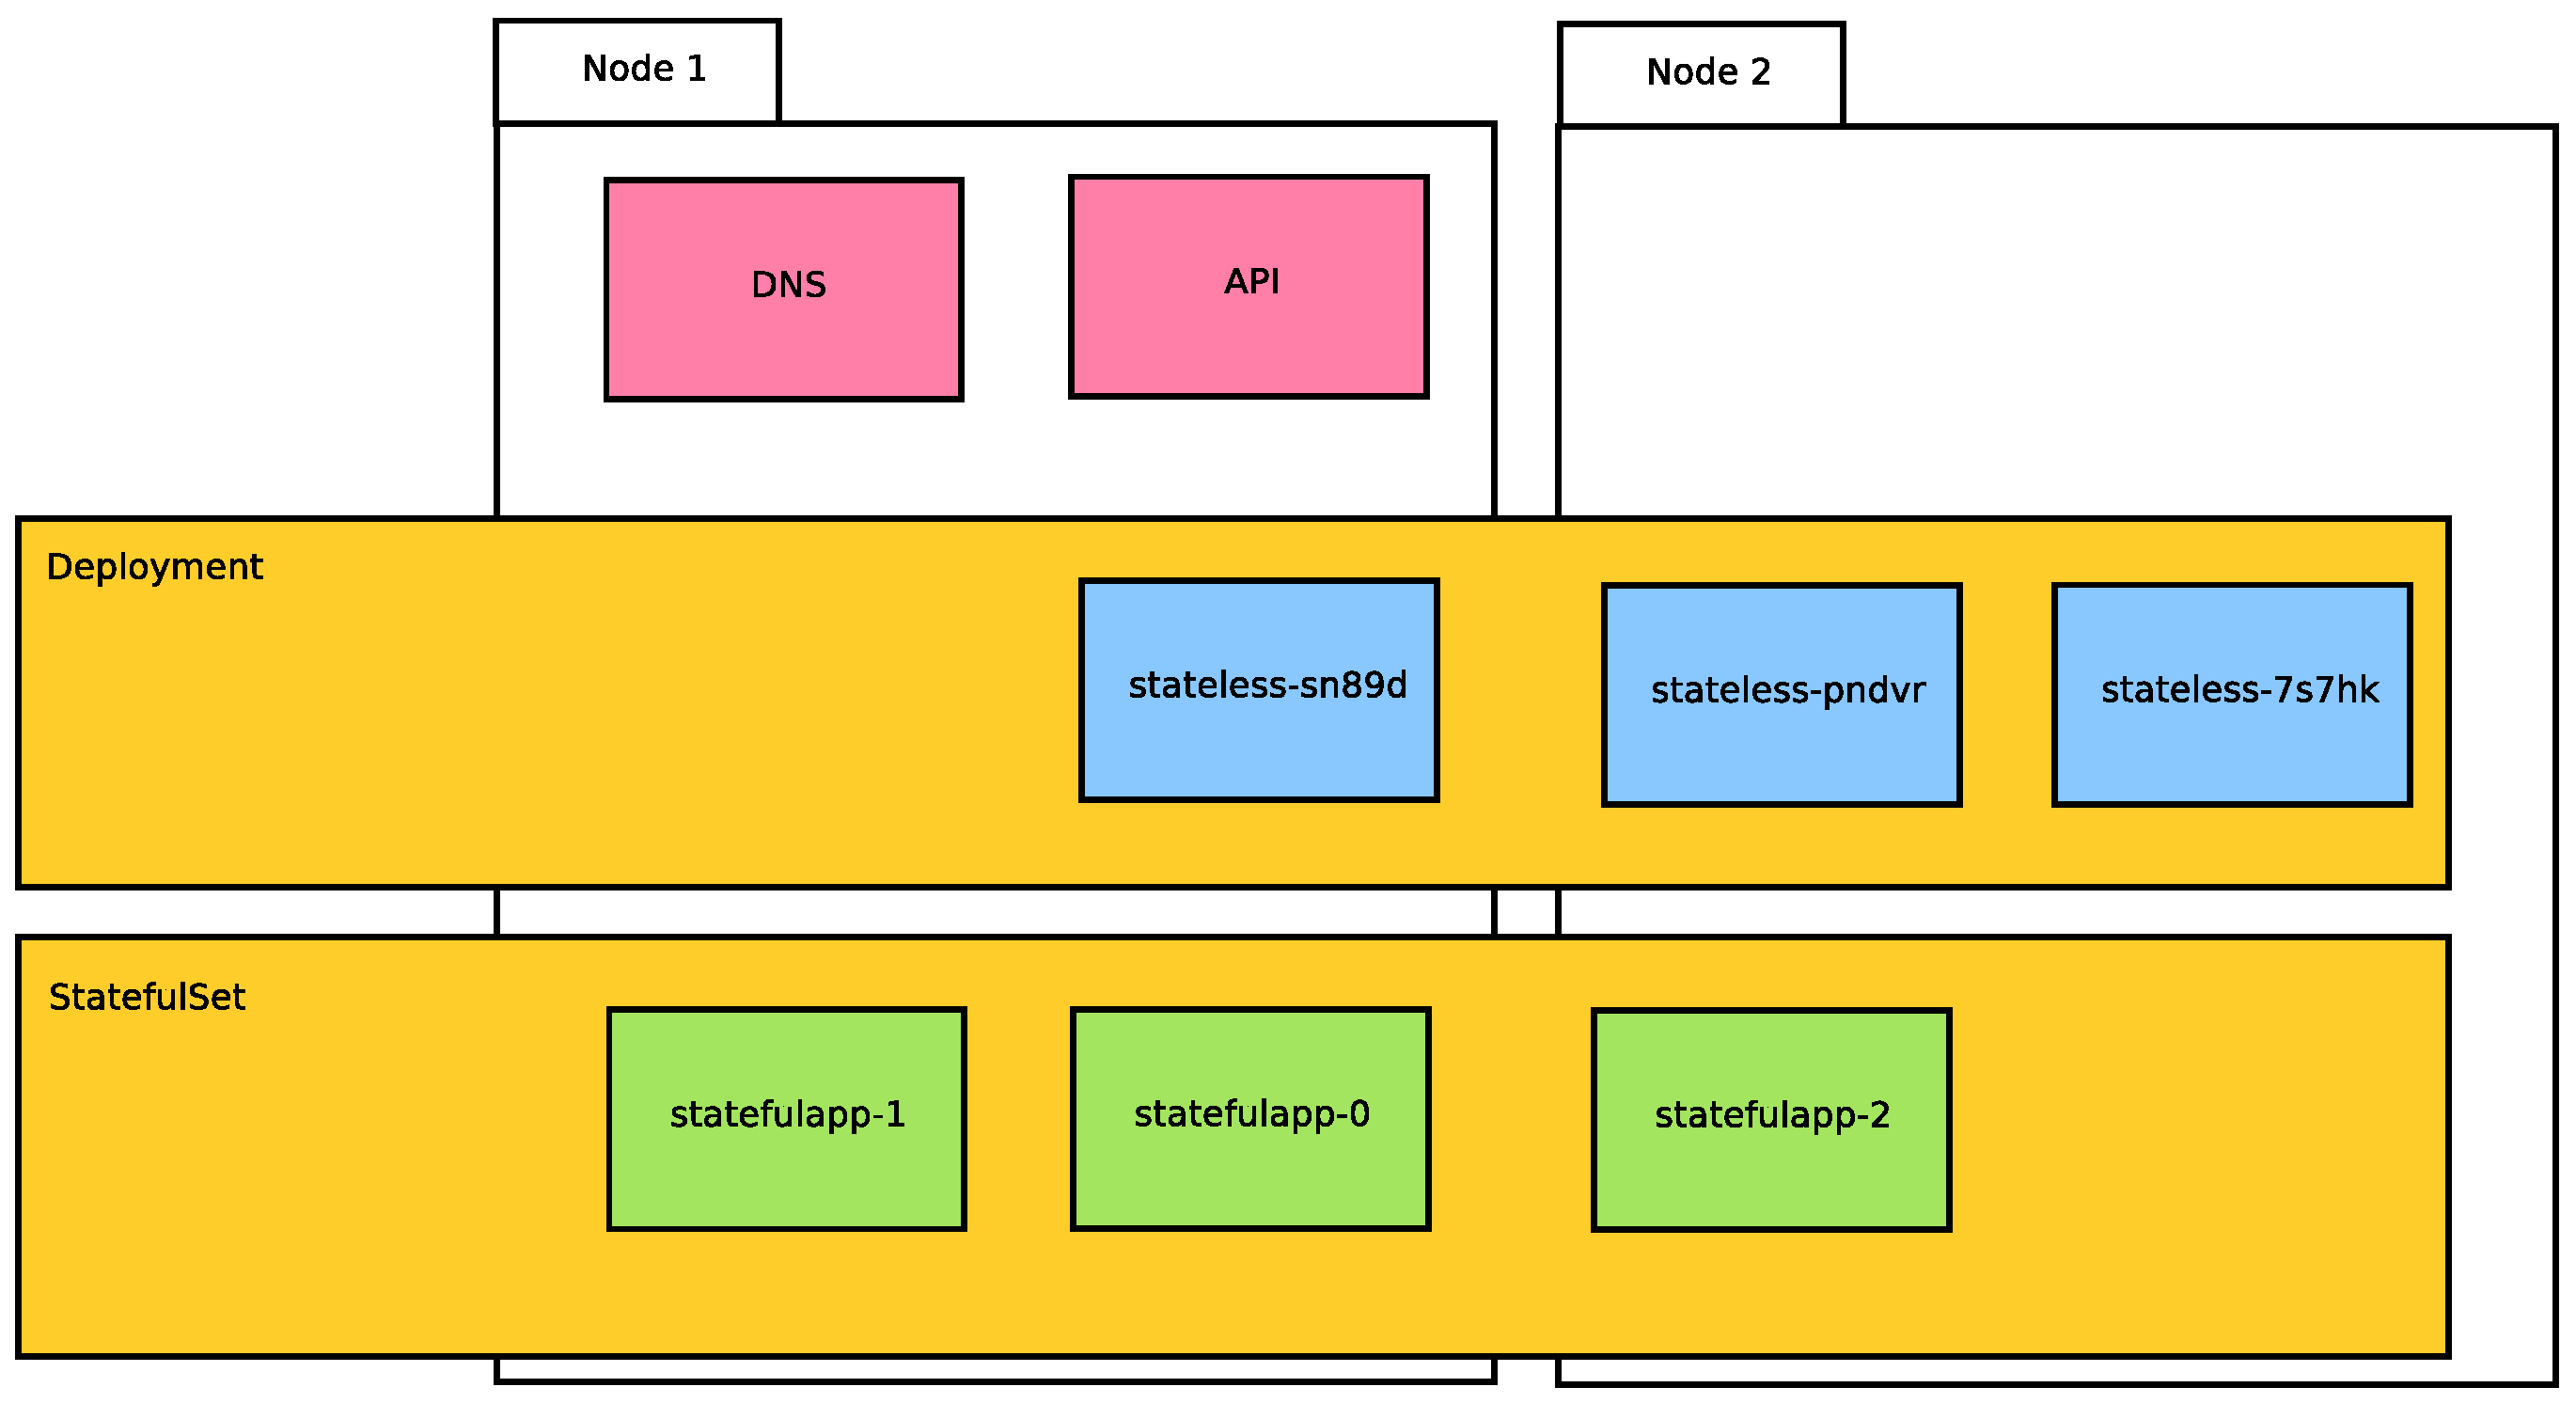
\includegraphics[width=\textwidth,height=0.85\textheight,keepaspectratio]{graphics/05-statefulSet.eps}
\end{frame}

\begin{frame}
    \frametitle{StatefulSet: Persistent Storage}
    \begin{itemize}
        \item StatefulSet Pods can have PersistentVolumeClaims (PVCs).
        \item PVCs are used to request PersistentVolumes.
        \item PersistentVolumes are Volumes that survive Pods being moved or replaced.
    \end{itemize}
\end{frame}

\begin{frame}
    \frametitle{StatefulSet: Persistent Storage}
    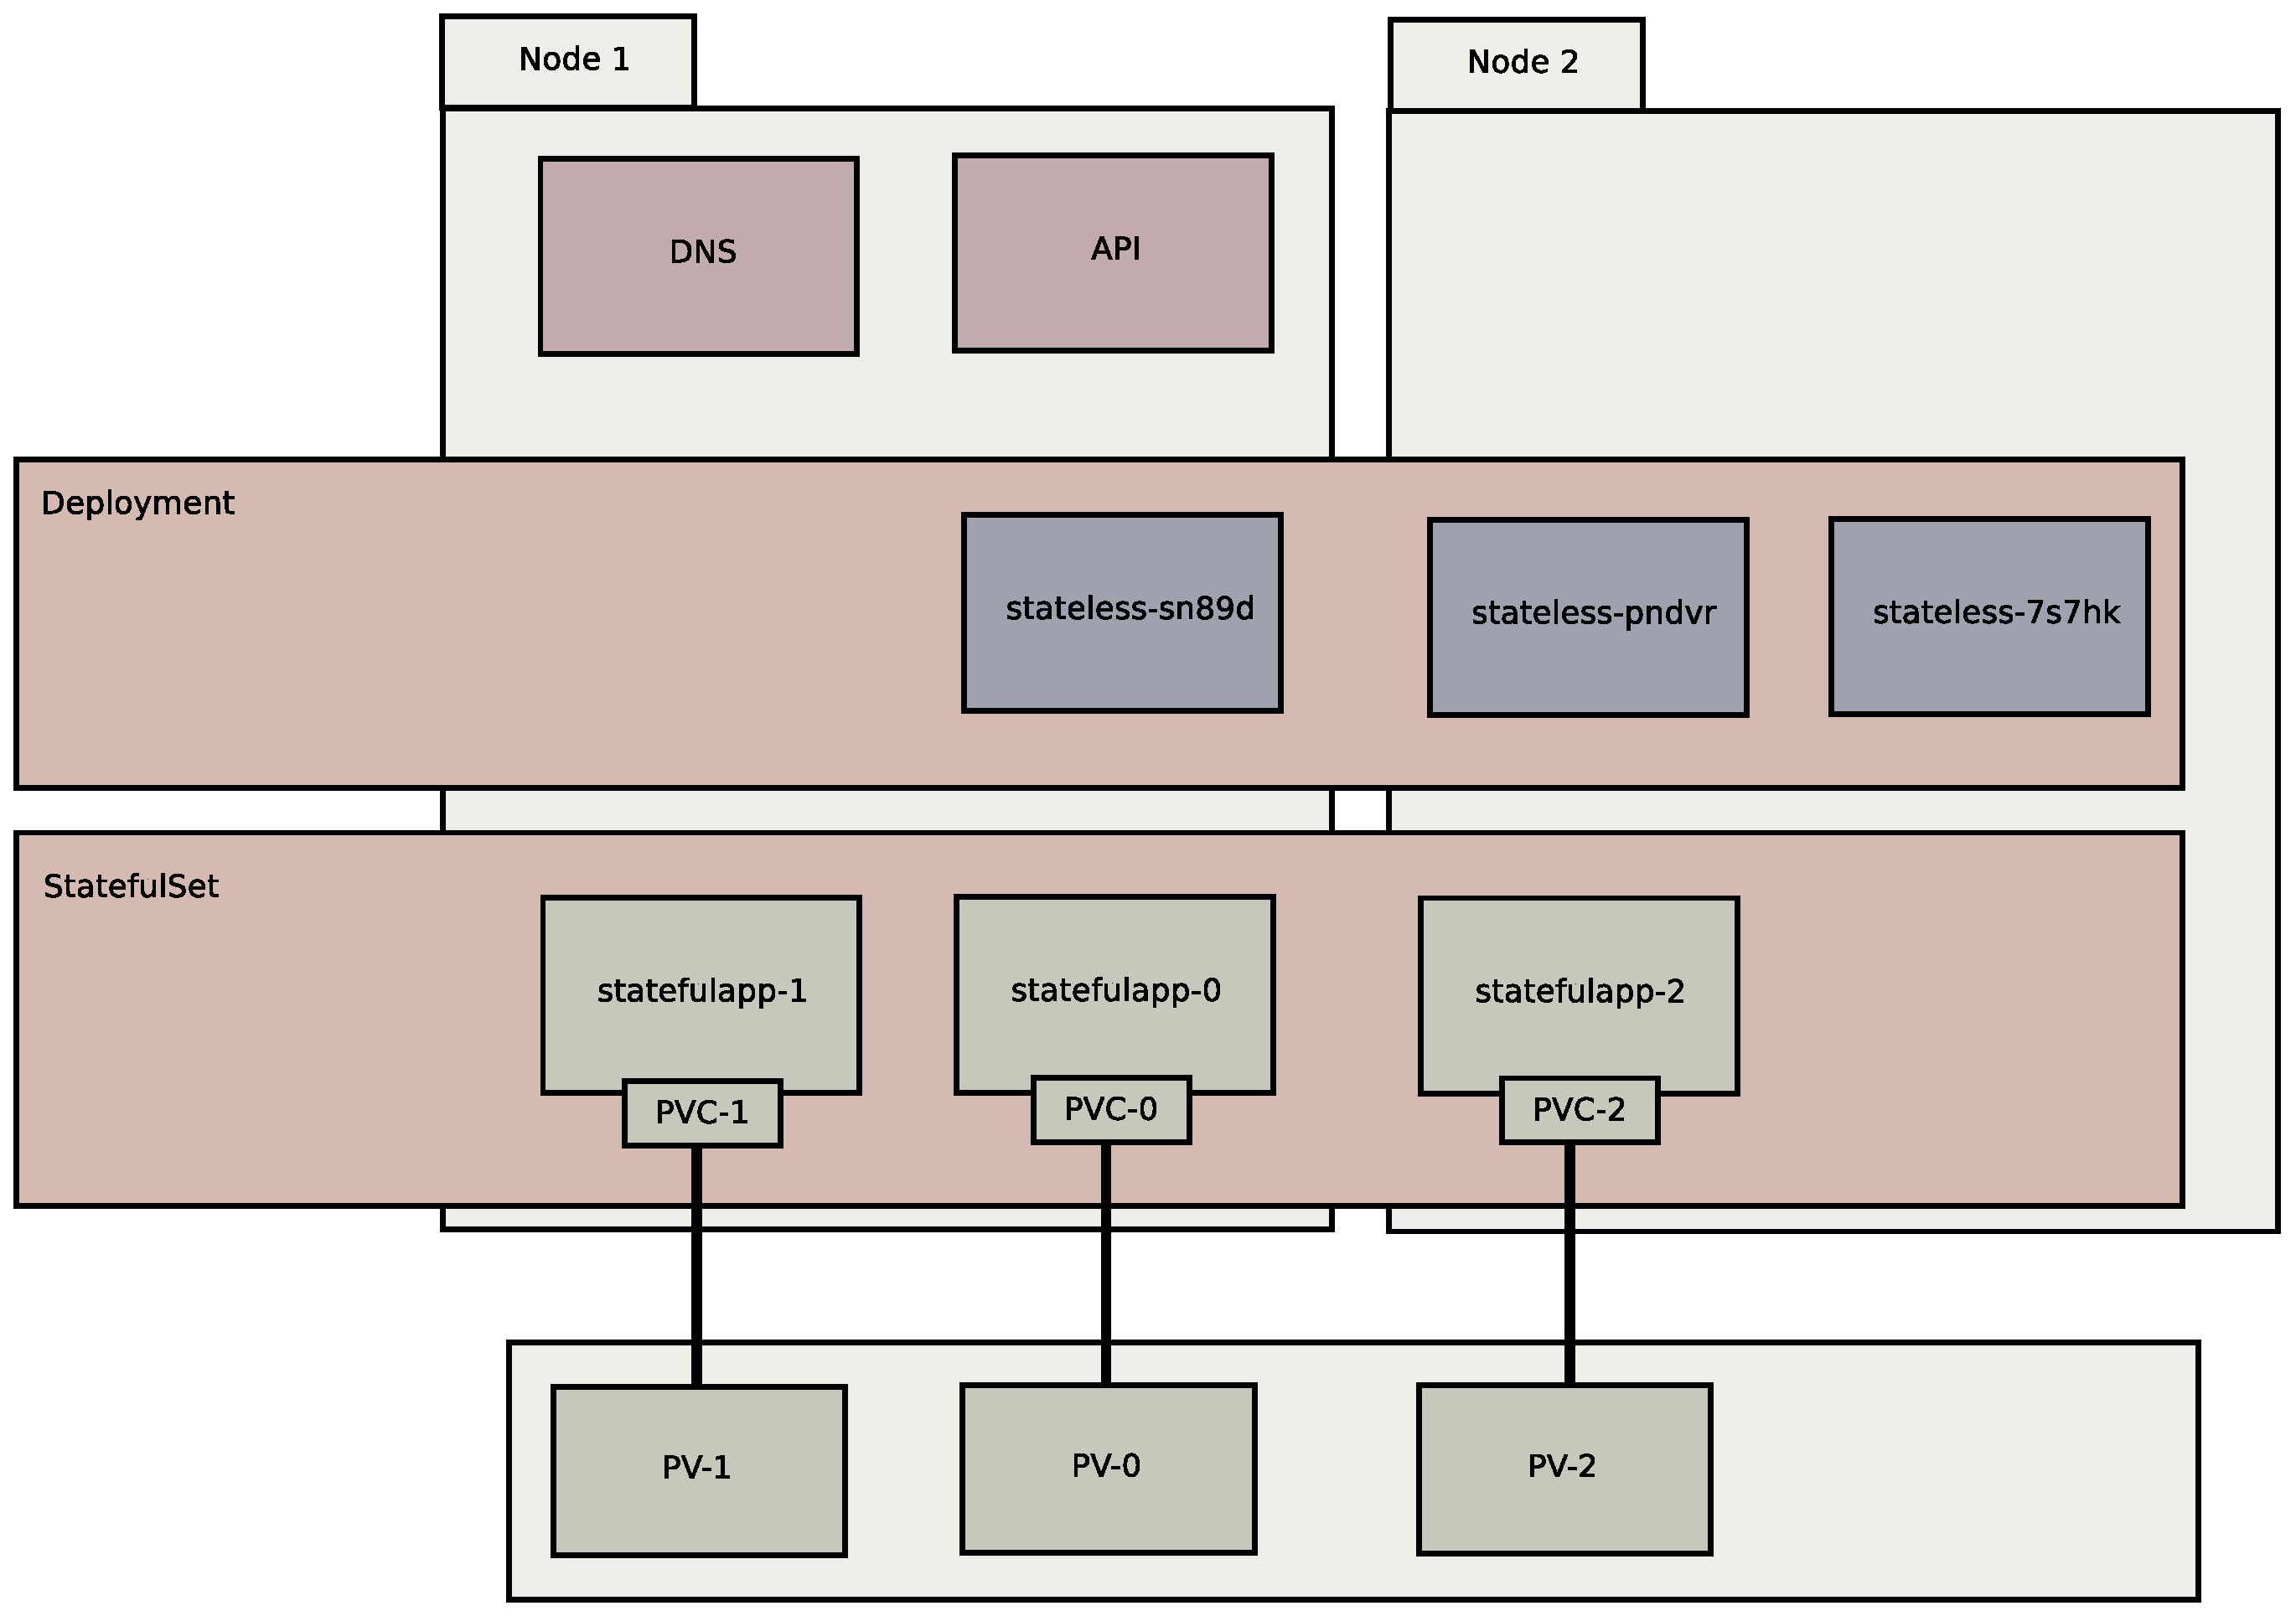
\includegraphics[width=\textwidth,height=0.85\textheight,keepaspectratio]{graphics/06-persistence.eps}
\end{frame}

\begin{frame}
    \frametitle{StatefulSet: Headless Service}
    StatefulSets require a Headless Service
    \begin{itemize}
        \item It's used by the Kubernetes DNS Pod.
        \item It allows Pods to keep their hostname by keeping track of their IP address (even when it changes).
    \end{itemize}
\end{frame}

\begin{frame}
    \frametitle{StatefulSet: Headless Service}
    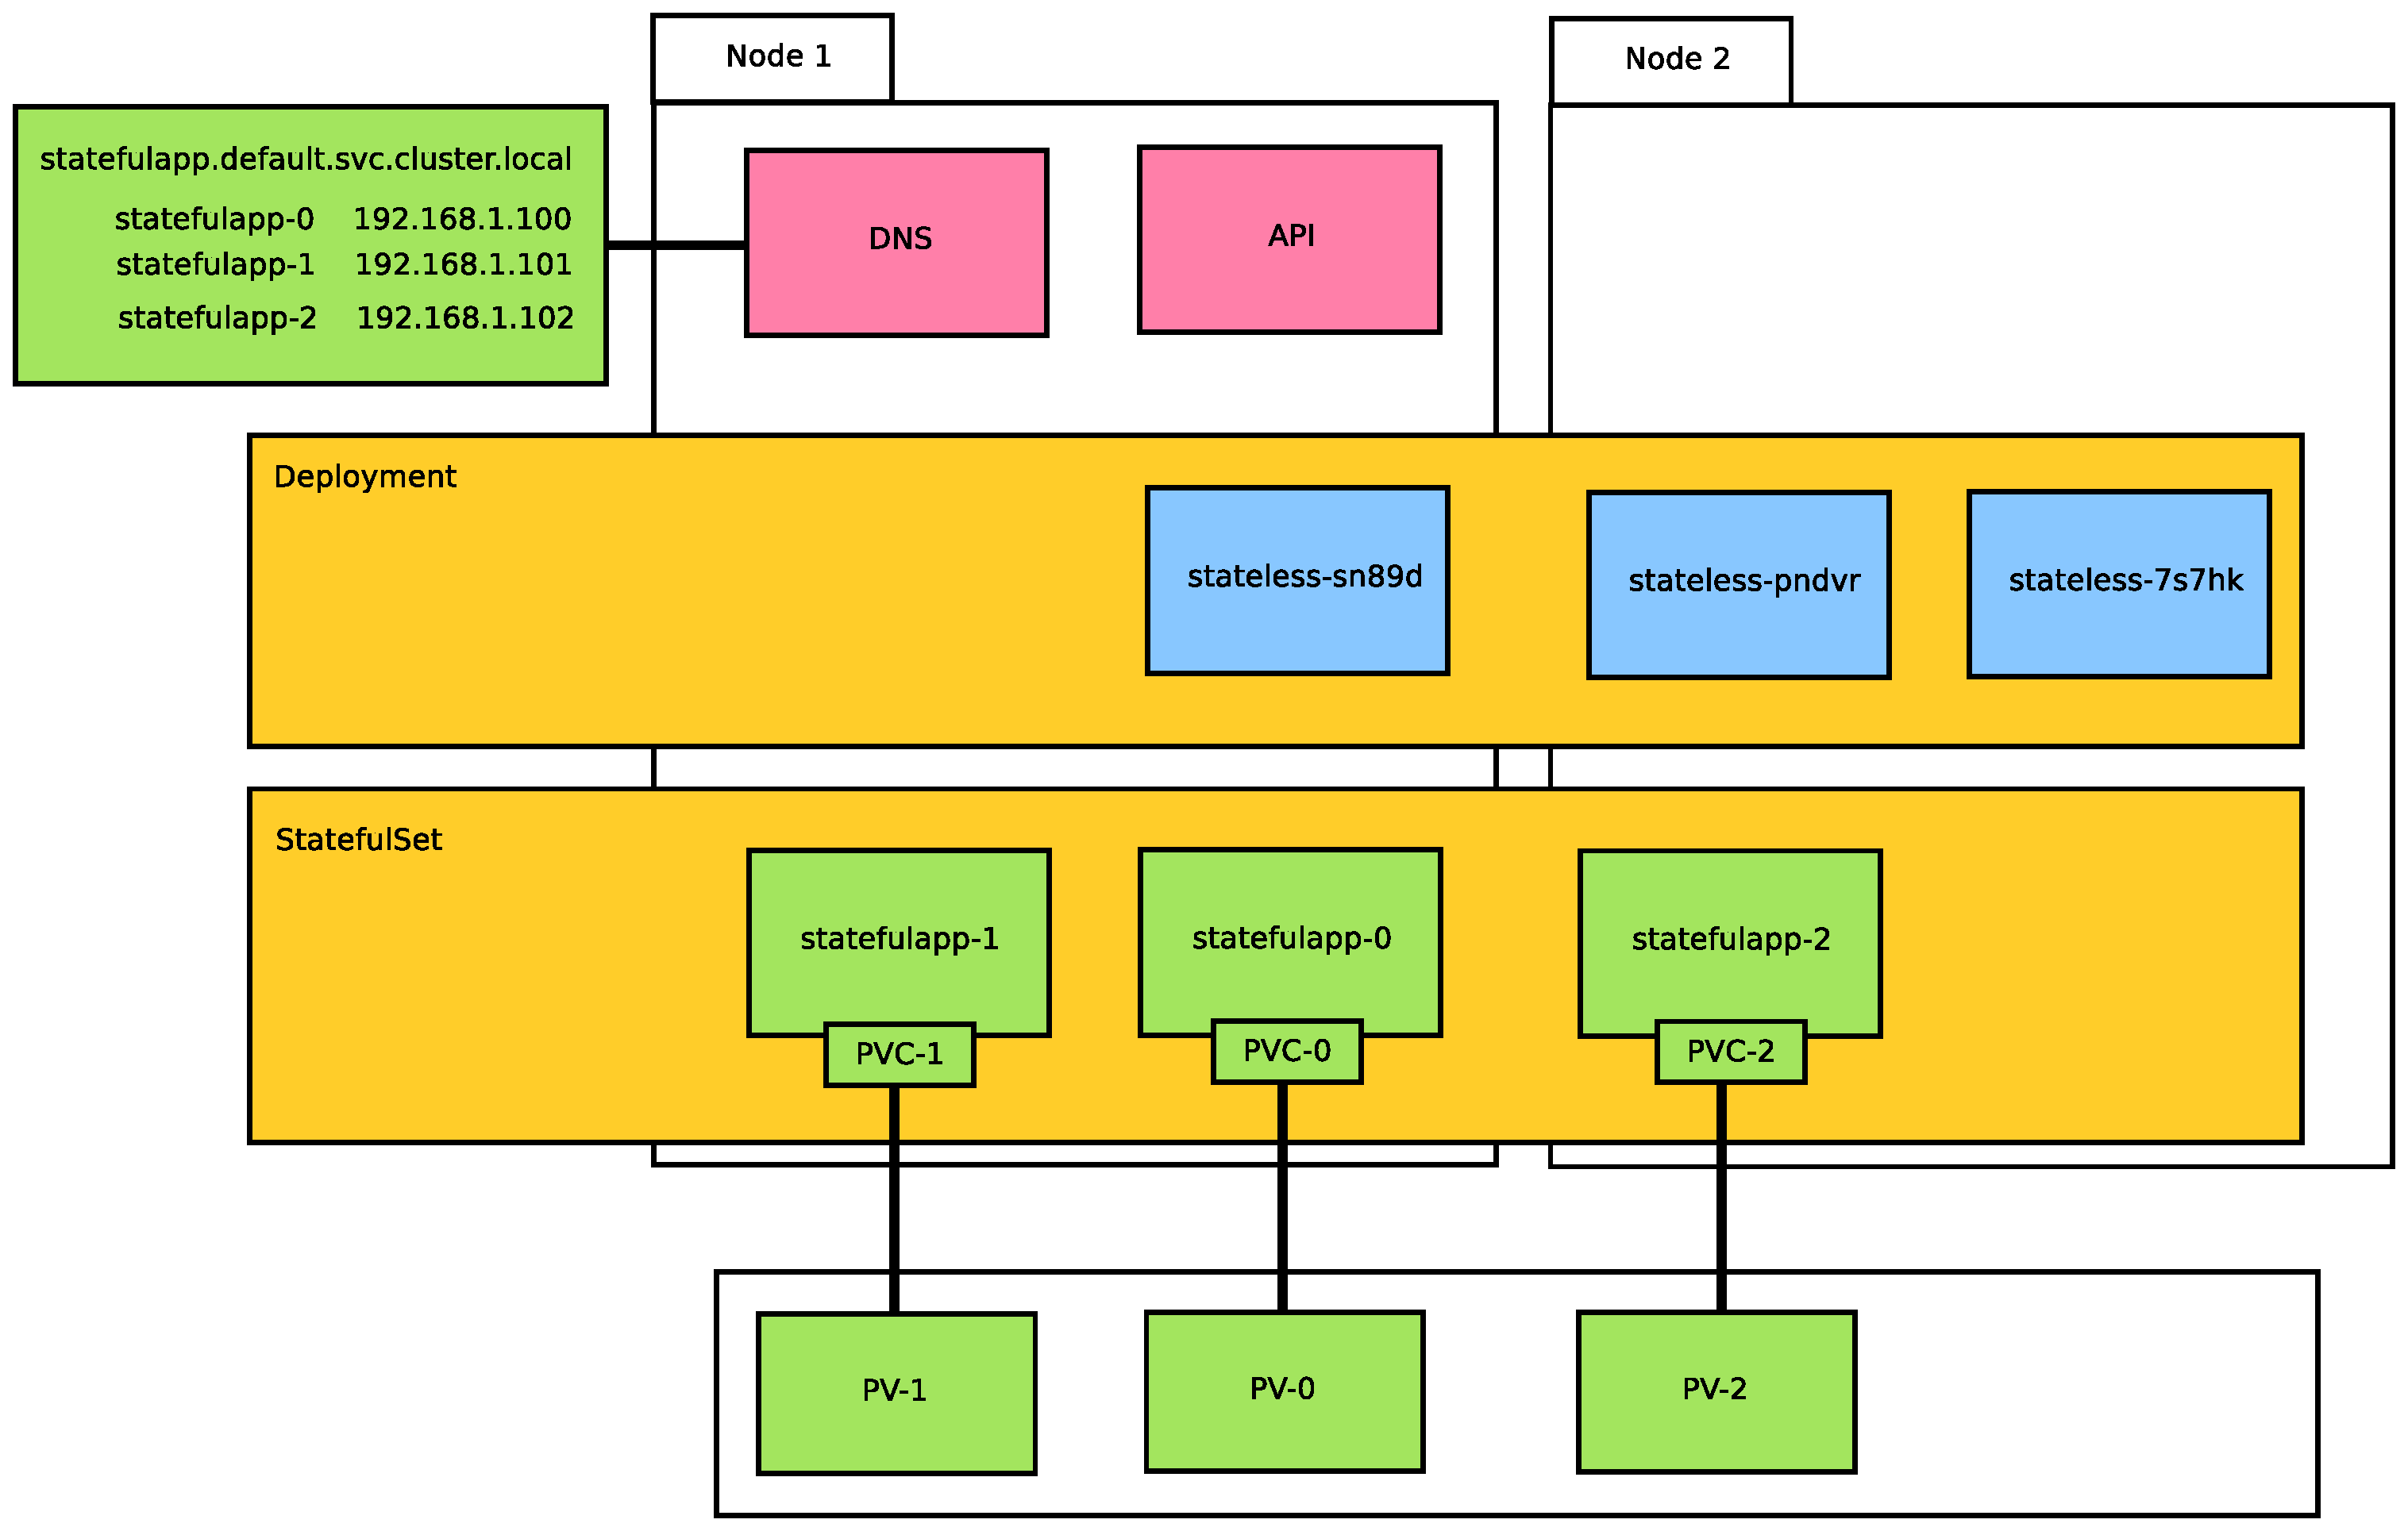
\includegraphics[width=\textwidth,height=0.85\textheight,keepaspectratio]{graphics/07-persistentIdentity.eps}
\end{frame}

\begin{frame}
    \frametitle{Load Balancers}
    \begin{itemize}
        \item Load Balancers have an internal cluster IP address.
        \item They can also have an external IP address.
        \item They distribute requests sent to either IP address to all Pods targeted by their ``selector".
    \end{itemize}
\end{frame}

\begin{frame}
    \frametitle{Load Balancers}
    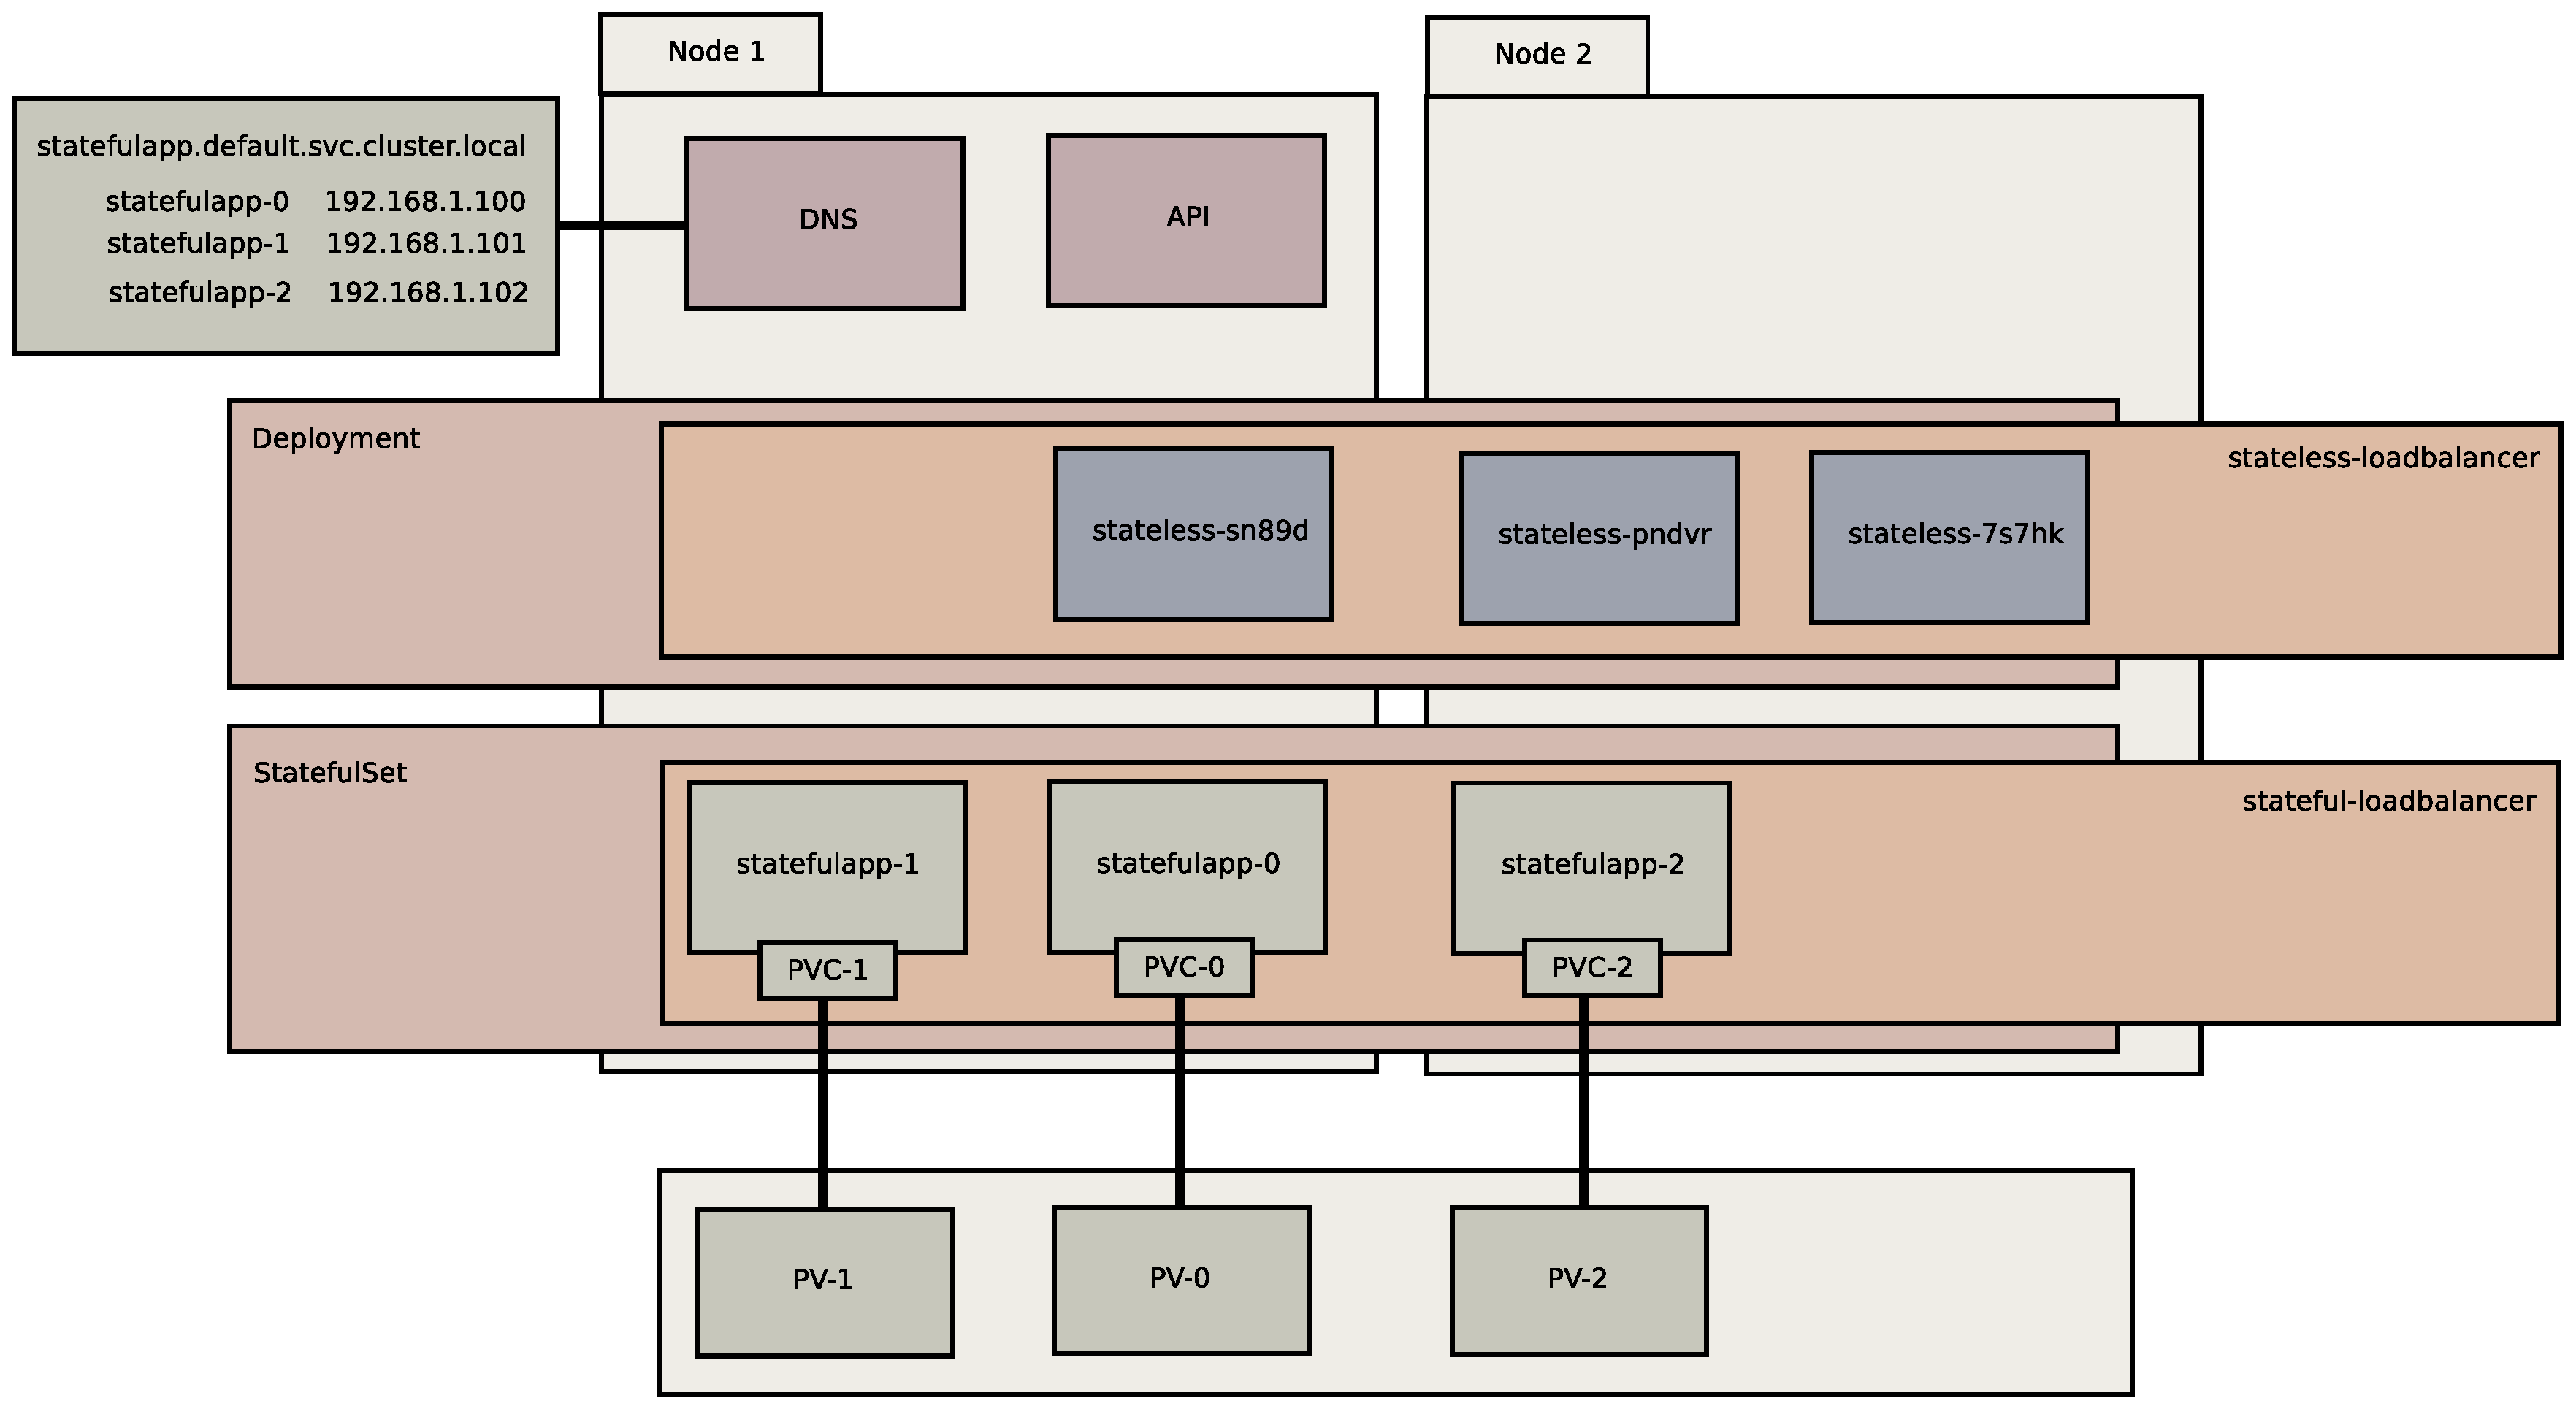
\includegraphics[width=\textwidth,height=0.85\textheight,keepaspectratio]{graphics/08-loadBalancer.eps}
\end{frame}

\begin{frame}
    \frametitle{Demo}
    \begin{center}
        \Huge So, let's see this in action!
    \end{center}
\end{frame}

\begin{frame}
    \frametitle{Overview}
    First, let's talk about the steps we're going to take:
    \begin{itemize}
        \item Start our Kubernetes environment (minikube).
        \item Configure our docker cli to talk to minikube's docker host.
        \item Build our two sample Applications, package them as docker Containers, and push the images.
        \item Run helm to deploy our Kubernetes components.
        \item Proxy local ports to connect to our load balancing services.
    \end{itemize}
\end{frame}

\begin{frame}
    \frametitle{Demo: Simplified Architecture}
    \includegraphics[width=\textwidth,height=0.85\textheight,keepaspectratio]{graphics/simplifiedModel-00.eps}
\end{frame}

\begin{frame}
    \begin{center}
        \Huge Is there enough time to go deeper?\\
        If so, let's dig into some code.
    \end{center}
\end{frame}

\begin{frame}
\frametitle{Other Resources}
Peripheral tools I used -- some of which warrant their own presentation
\begin{itemize}
    \item \LaTeX: \href{https://www.latex-project.org}{https://www.latex-project.org}
    \item Beamer: \href{https://ctan.org/pkg/beamer}{https://ctan.org/pkg/beamer}
    \item Kotlin: \href{https://kotlinlang.org}{https://kotlinlang.org}
    \item Spring Boot: \href{https://spring.io/projects/spring-boot}{https://spring.io/projects/spring-boot}
    \item Gradle: \href{https://gradle.org}{https://gradle.org}
    \item Dia: \href{http://dia-installer.de}{http://dia-installer.de}
\end{itemize}
\smallskip
Where I got my Subreddit data
\begin{itemize}
    \item Bulk Reddit data: \href{http://files.pushshift.io/reddit/subreddits}{http://files.pushshift.io/reddit/subreddits}
\end{itemize}
Finally, \textbf{\textit{this}} demo
\begin{itemize}
    \item \href{https://github.com/emacdona/k8sdemo}{https://github.com/emacdona/k8sdemo}
\end{itemize}
\end{frame}

\begin{frame}
    \begin{center}
        \Huge Questions?
    \end{center}
\end{frame}

\end{document}
